%===========================================================
\documentclass[10pt]{article}
\usepackage[a4paper]{geometry}
\usepackage[T1]{fontenc}
\usepackage{graphicx}
\usepackage{alltt}
\usepackage{caption}
\usepackage{hyperref}
\captionsetup[figure]{labelformat=empty}
\captionsetup[table]{labelformat=empty}

\pagestyle{plain}
\thispagestyle{plain}
%===========================================================
%                          Title
%===========================================================
\title{HBF-701 Unofficial English Manual}
\author{Peter Senna Tschudin\footnote{I do not work for Omron. I just own one
HBF-701}\\ {\small peter.senna@gmail.com}}
\begin{document}
\maketitle
%===========================================================
%                          Title
%===========================================================
\begin{center}
\vspace{-30pt}
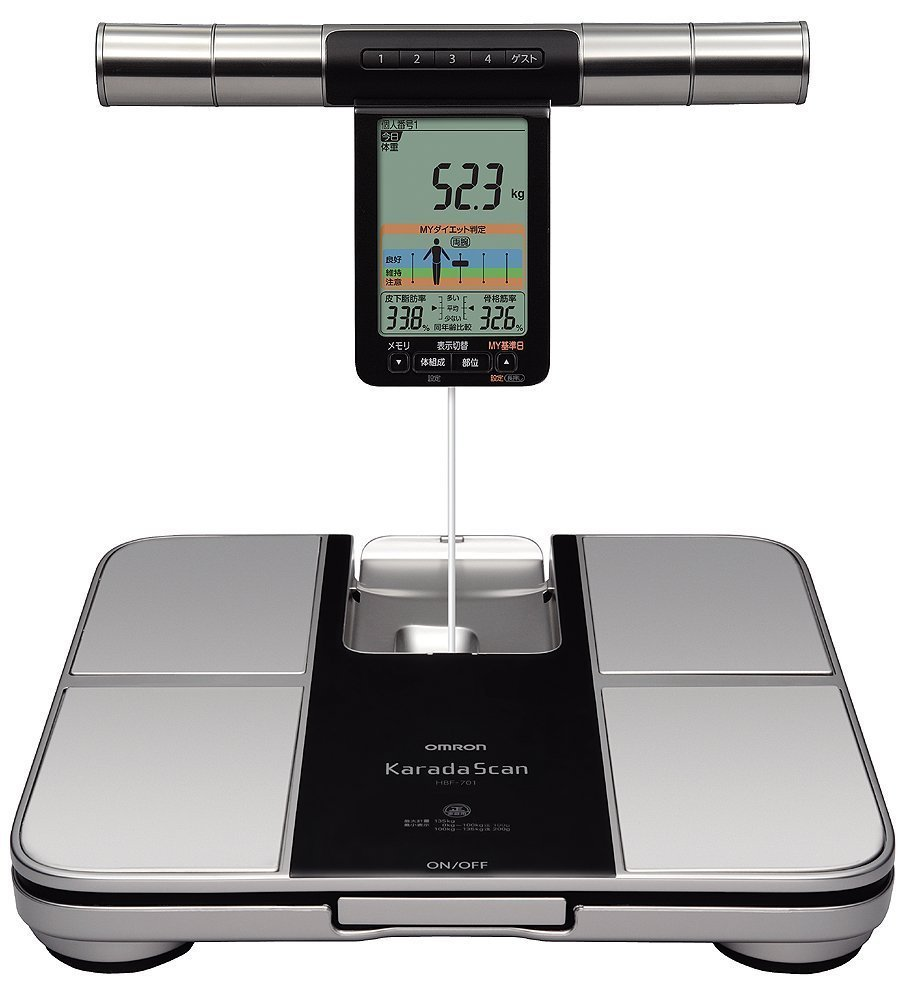
\includegraphics[width=0.8\linewidth]{images/hbf701.jpg}
\end{center}
\section{Getting started}
\label{sec:starting}
\section{Legal notice}
\label{sec:legal}
\begin{itemize}
  \item I do not work for Omron. I just own one HBF-701
  \item All trademarks and/or brands cited in this document, including but not
        limited to ``Omron'' are property of their respespective owners
  \item The official manual in Japanese is available at:
        \url{http://www.healthcare.omron.co.jp/product/hbf/hbf-701.html}
  \item This work is licensed under a Creative Commons Attribution 4.0
        International License
\end{itemize}
\end{document}
